\documentclass[tikz,border=10pt]{standalone}
\usepackage{tikz}
\usetikzlibrary{arrows.meta,positioning,fit,backgrounds,calc,decorations.pathreplacing}

\definecolor{l0color}{HTML}{E8F4FD}
\definecolor{l1color}{HTML}{D1E7DD}
\definecolor{l2color}{HTML}{FFF3CD}
\definecolor{l3color}{HTML}{F8D7DA}
\definecolor{gatecolor}{HTML}{6C757D}
\definecolor{denycolor}{HTML}{DC3545}
\definecolor{allowcolor}{HTML}{198754}
\definecolor{ceremonycolor}{HTML}{0D6EFD}

\begin{document}
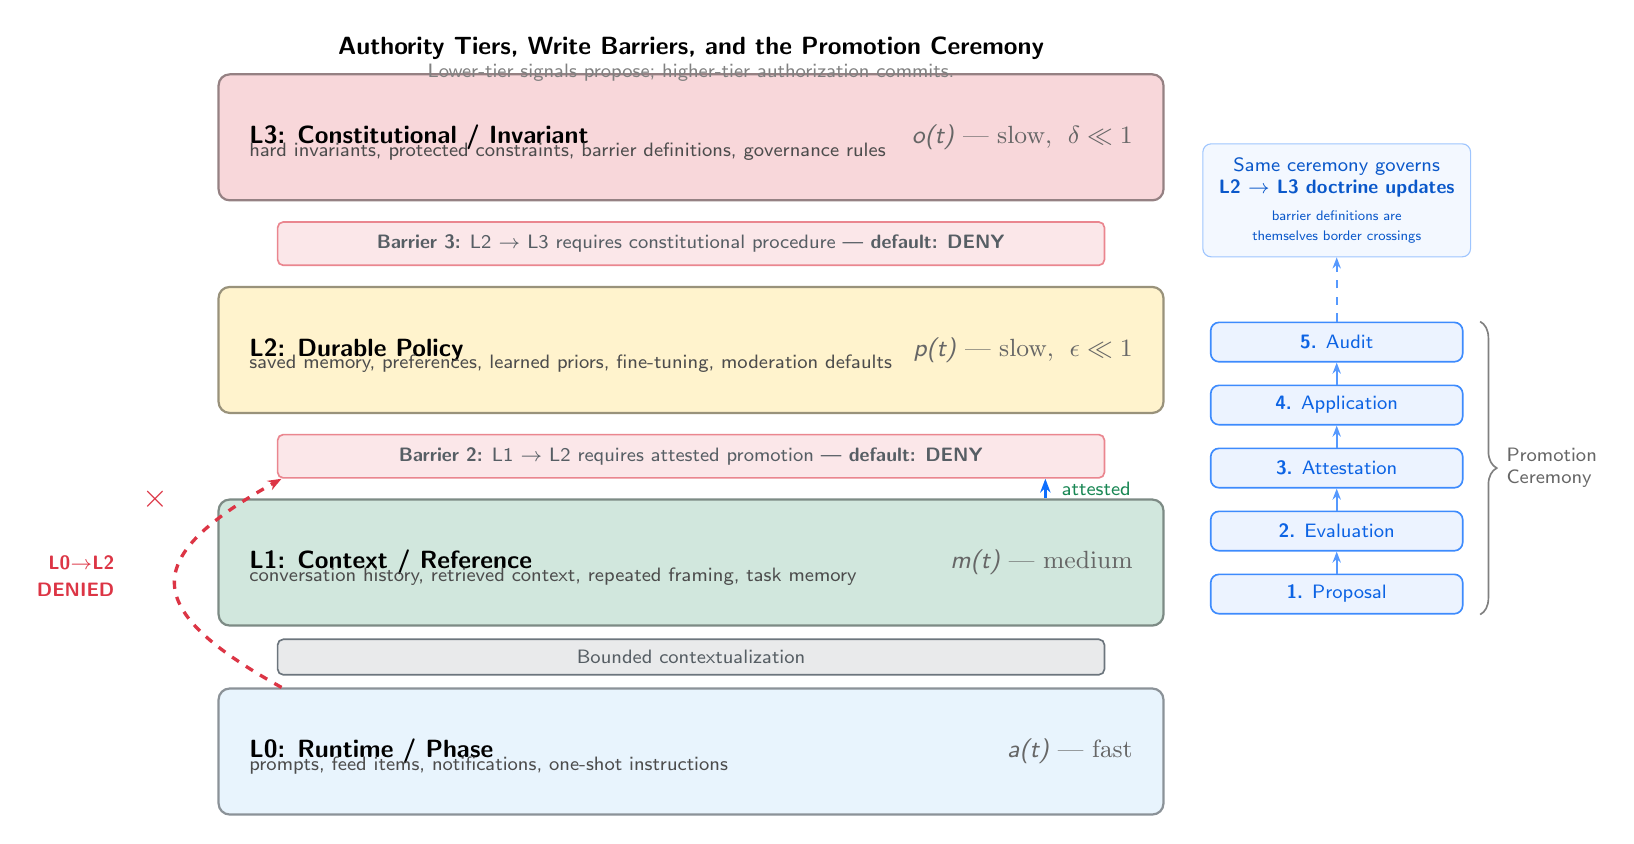
\begin{tikzpicture}[
    tier/.style={
        rectangle, rounded corners=4pt, minimum width=12cm, minimum height=1.6cm,
        draw=#1!60!black, line width=0.8pt, fill=#1, font=\sffamily
    },
    tierlabel/.style={
        font=\sffamily\bfseries\small, anchor=west
    },
    tierdetail/.style={
        font=\sffamily\scriptsize, anchor=west, text=black!70
    },
    statevar/.style={
        font=\sffamily\small\itshape, anchor=east, text=black!60
    },
    barrier/.style={
        rectangle, rounded corners=2pt, minimum width=10.5cm, minimum height=0.45cm,
        draw=gatecolor, line width=0.6pt, fill=gatecolor!15,
        font=\sffamily\scriptsize, text=gatecolor!80!black
    },
    denied/.style={
        -{Stealth[length=5pt]}, line width=1.2pt, color=denycolor, dashed
    },
    attested/.style={
        -{Stealth[length=5pt]}, line width=1.2pt, color=allowcolor
    },
    ceremony/.style={
        rectangle, rounded corners=3pt, minimum width=2.8cm, minimum height=0.5cm,
        draw=ceremonycolor!80, line width=0.6pt, fill=ceremonycolor!8,
        font=\sffamily\scriptsize, text=ceremonycolor!90!black
    },
    ceremonyarrow/.style={
        -{Stealth[length=4pt]}, line width=0.7pt, color=ceremonycolor!70
    },
    brace/.style={
        decorate, decoration={brace, amplitude=6pt, raise=2pt},
        line width=0.6pt, draw=black!50
    },
    bracelabel/.style={
        font=\sffamily\scriptsize, text=black!60
    }
]

% Tiers (bottom to top)
\node[tier=l0color] (L0) at (0, 0) {};
\node[tierlabel] at ([xshift=8pt]L0.west) {L0: Runtime / Phase};
\node[tierdetail] at ([xshift=8pt, yshift=-5pt]L0.west) {prompts, feed items, notifications, one-shot instructions};
\node[statevar] at ([xshift=-8pt]L0.east) {a(t) \textnormal{--- fast}};

% Barrier L0-L1
\node[barrier] (B01) at (0, 1.2) {Bounded contextualization};

\node[tier=l1color] (L1) at (0, 2.4) {};
\node[tierlabel] at ([xshift=8pt]L1.west) {L1: Context / Reference};
\node[tierdetail] at ([xshift=8pt, yshift=-5pt]L1.west) {conversation history, retrieved context, repeated framing, task memory};
\node[statevar] at ([xshift=-8pt]L1.east) {m(t) \textnormal{--- medium}};

% Barrier L1-L2 (the big one)
\node[barrier, minimum height=0.55cm, fill=denycolor!12, draw=denycolor!60] (B12) at (0, 3.75) {\textbf{Barrier 2:} L1 $\to$ L2 requires attested promotion --- \textbf{default: DENY}};

\node[tier=l2color] (L2) at (0, 5.1) {};
\node[tierlabel] at ([xshift=8pt]L2.west) {L2: Durable Policy};
\node[tierdetail] at ([xshift=8pt, yshift=-5pt]L2.west) {saved memory, preferences, learned priors, fine-tuning, moderation defaults};
\node[statevar] at ([xshift=-8pt]L2.east) {p(t) \textnormal{--- slow,\;} $\epsilon \ll 1$};

% Barrier L2-L3
\node[barrier, minimum height=0.55cm, fill=denycolor!12, draw=denycolor!60] (B23) at (0, 6.45) {\textbf{Barrier 3:} L2 $\to$ L3 requires constitutional procedure --- \textbf{default: DENY}};

\node[tier=l3color] (L3) at (0, 7.8) {};
\node[tierlabel] at ([xshift=8pt]L3.west) {L3: Constitutional / Invariant};
\node[tierdetail] at ([xshift=8pt, yshift=-5pt]L3.west) {hard invariants, protected constraints, barrier definitions, governance rules};
\node[statevar] at ([xshift=-8pt]L3.east) {o(t) \textnormal{--- slow,\;} $\delta \ll 1$};

% Denied arrow: L0 direct to L2 (single arc, bypassing L1)
\draw[denied] ([xshift=-5.2cm]L0.north)
    .. controls ([xshift=-7cm, yshift=1cm]L0.north) and ([xshift=-7cm, yshift=-1cm]B12.south)
    .. ([xshift=-5.2cm]B12.south);
\node[font=\sffamily\scriptsize\bfseries, text=denycolor, anchor=east] at ([xshift=-7.2cm]$(L1)$) {L0$\to$L2};
\node[font=\sffamily\scriptsize\bfseries, text=denycolor, anchor=east] at ([xshift=-7.2cm, yshift=-10pt]$(L1)$) {DENIED};

% X mark on the denied arrow
\node[font=\bfseries\large, text=denycolor] at ([xshift=-6.8cm]$(L1)!0.6!(B12)$) {$\times$};

% Promotion ceremony (right side)
\node[ceremony, minimum width=3.2cm] (C1) at (8.2, 2.0) {\textbf{1.} Proposal};
\node[ceremony, minimum width=3.2cm] (C2) at (8.2, 2.8) {\textbf{2.} Evaluation};
\node[ceremony, minimum width=3.2cm] (C3) at (8.2, 3.6) {\textbf{3.} Attestation};
\node[ceremony, minimum width=3.2cm] (C4) at (8.2, 4.4) {\textbf{4.} Application};
\node[ceremony, minimum width=3.2cm] (C5) at (8.2, 5.2) {\textbf{5.} Audit};

\draw[ceremonyarrow] (C1) -- (C2);
\draw[ceremonyarrow] (C2) -- (C3);
\draw[ceremonyarrow] (C3) -- (C4);
\draw[ceremonyarrow] (C4) -- (C5);

% Brace around ceremony
\draw[brace] ([xshift=4pt]C5.north east) -- ([xshift=4pt]C1.south east);
\node[bracelabel, anchor=west, align=left] at ([xshift=12pt]$(C3.east)$) {Promotion\\Ceremony};

% Arrow from L1 through ceremony to L2
\draw[attested, ceremonycolor] ([xshift=4.5cm]L1.north) -- ([xshift=4.5cm]B12.south)
    node[midway, right, font=\sffamily\scriptsize, text=allowcolor, xshift=2pt] {attested};

% Recursive governance note
\node[rectangle, rounded corners=3pt, draw=ceremonycolor!40, fill=ceremonycolor!5,
      minimum width=3.4cm, align=center, font=\sffamily\scriptsize,
      text=ceremonycolor!80!black, inner sep=5pt] (recursive) at (8.2, 7.0) {
    Same ceremony governs\\
    \textbf{L2 $\to$ L3 doctrine updates}\\[2pt]
    {\tiny barrier definitions are}\\[-1pt]
    {\tiny themselves border crossings}
};
\draw[ceremonyarrow, dashed] (C5.north) -- (recursive.south);

% Title
\node[font=\sffamily\bfseries\small, anchor=north] at (0, 9.2) {Authority Tiers, Write Barriers, and the Promotion Ceremony};

% Subtitle
\node[font=\sffamily\scriptsize, text=black!50, anchor=north] at (0, 8.85) {Lower-tier signals propose; higher-tier authorization commits.};

\end{tikzpicture}
\end{document}
